\section{Diseño del circuito} 
\subsection{Esquemático}
El diseño del hardware se muestra en la figura \ref{Fig: Diseño}. Por un lado, para la conversión de tensión de $[\SI{-24}{\volt}, \SI{24}{\volt}]$ a $[\SI{0}{\volt}, \SI{5}{\volt}]$ se utiliza una red resistiva con una fuente de tensión DC \cite{electronics-stackexchange}. Por otro lado, los switches en el lado izquerdo ya están con las resistencias de \it{pull-up}, que están dentro del Arduino UNO \cite{pullup}. Finalmente, por instrucciones de Carlos Rodríguez \cite{pcd}, la pantalla está conectado de esa manera y los LEDs rojos son protegidos por resistencias. 
\begin{figure}[H]
\centering
\includegraphics[width=0.9\textwidth]{Imagenes/Diseno_circuito.png} 
\caption{Diseño del circuito.}
\label{Fig: Diseño}
\end{figure}

\subsection{Disminución del efecto rebote de los switches}
De acuerdo con la información de referencia del Arduino UNO, el microcontrolador tiene resistencias de \it{pull-up} internas de \SI{20}{\kilo\ohm} \cite{pullup}.
La obtención de estos valores de resistencias y el valor de la capacitancia se da por medio de la ecuación
\begin{equation}
    \tau = RC.
\end{equation}
Como el interruptor oscila entre estar cerrado y abierto entre diez a cien veces en un periodo de \SI{1}{\milli\second}, se puede llegar a despejar la capacitancia $C$
\cite{boton},
\begin{equation*}
    C = \frac{\tau}{R} = \frac{\SI{1}{\milli\second}}{\SI{20}{\kilo\ohm}} = \SI{50}{\nano\farad}.
\end{equation*}

Por lo tanto, se decide utilizar una capacitancia de \SI{47}{\nano\farad}, ya que es el valor comercial más cercano.
 

 
\subsection{Cálculo de las resistencias}
Ahora, la figura \ref{Fig: cal_resist} ilustra la red resistiva  que ``convierte'' tensiones entre \SI{-24}{\volt} a \SI{24}{\volt} a un rango entre \SI{0}{\volt} a \SI{5}{\volt}, que es el rango de tensión que puede soportar el Arduino UNO. Para una tensión de entrada máximo de $V_\text{i max} = \SI{24}{\volt}$ y mínima de $V_\text{i min} = \SI{-24}{\volt}$, así como una tensión de salida máxima de $V_\text{o} = \SI{5}{\volt}$, los valores de las resistencias deben ser
\begin{align}
    R_3 &= \frac{R_1 \cdot V_\text{o}}{V_\text{i max} - V_\text{o}}\\
    R_2 &= \frac{R_1 \cdot V_\text{o}}{|V_\text{i min}|},
\end{align}
siendo $R_1$ un valor arbitrario \cite{electronics-stackexchange}. Por lo tanto, para un $R_1 = \SI{10}{\kilo\ohm}$, $R_2$ y $R_3$ deben ser
\begin{align*}
    R_3 &\approx \SI{2.631}{\kilo\ohm}\\
    R_2 &\approx \SI{2.083}{\kilo\ohm}.
\end{align*}
Se escogerán resistencias comerciales de \SI{1.8}{\kilo\ohm} y \SI{820}{\ohm} para $R_3$ y de \SI{1.8}{\kilo\ohm} y \SI{270}{\ohm} para $R_2$ puesto que son la combinación de resistencias más cercanas a los valores teóricos, respectivamente.

\begin{figure}[H]
\centering
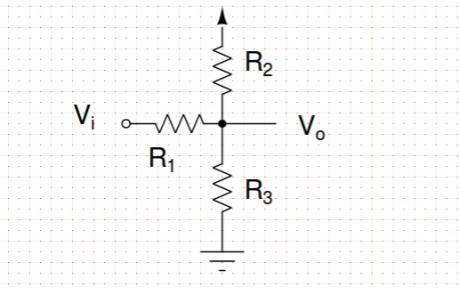
\includegraphics[width=0.6\textwidth]{Imagenes/Calculos_Resistecias.jpg} 
\caption{Red resistiva para convertir el rango de la tensión de entrada a un rango apto para el Arduino UNO. Fuente y créditos: \cite{electronics-stackexchange}.}
\label{Fig: cal_resist}
\end{figure}

\subsubsection{Resistencia para un diodo LED Rojo}

\begin{figure}[H]
\centering
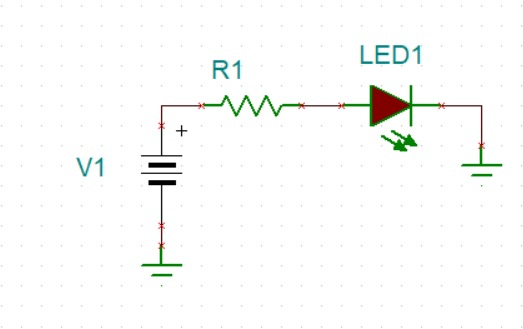
\includegraphics[width=0.55\textwidth]{Imagenes/Resistencia_LED_Rojo.jpg} 
\caption{Diagrama para calcular las resistencias de protección con el LED Rojo.}
\label{Fig: Diagrama 1}
\end{figure}

Se decide utilizar una corriente de \SI{10}{\milli\ampere}, ya que los diodos aceptan una corriente hasta de \SI{20}{\milli\ampere}. Por la hoja de fabricante se sabe que para los diodos LED's de color rojo el voltaje es de \SI{2.2}{\volt}. Con base en esa información se realizaron los siguientes cálculos: 

\begin{align}
    & V_{CC} = V_\text{R} + V_\text{D rojo}\\
    \Rightarrow& \SI{5}{\volt} = V_\text{R} + \SI{2.2}{\volt}\nonumber\\
    \Rightarrow& V_\text{R} = \SI{2.8}{\volt}.\nonumber
\end{align}
Ahora, por ley de Ohm
\begin{align}
    & V_\text{R} = I_\text{R} \cdot R\\
    \Rightarrow& R = \frac{V_\text{R}}{I_\text{R}} = \frac{\SI{2.8}{\volt}}{\SI{10}{\milli\ampere}} = \SI{280}{\ohm}. \nonumber
\end{align}

La resistencias con valor comercial mas cercano seria una resistencia de \SI{270}{\ohm}, por lo tanto, se cambia la \SI{280}{\ohm} por \SI{270}{\ohm}.

